\documentclass[8pt,a4paper,compress,handout]{beamer}

\usepackage{/home/siyer/lib/slides}

\title{Building a Computer}
\date{}

\begin{document}
\begin{frame}
\vfill
\titlepage
\end{frame}

\begin{frame}
\frametitle{Outline}
\tableofcontents
\end{frame}

\section{Boolean Algebra and Functions}
\begin{frame}[fragile]
\emph{Boolean variables} are variables that take the value \lstinline{True} (1) or \lstinline{False} (0).

\bigskip

With booleans 1 and 0 we could use the operations (functions) \lstinline{AND}, \lstinline{OR}, and \lstinline{NOT} to build up more interesting boolean functions.

\bigskip

A \emph{truth table} for a boolean function is a listing of all possible combinations of values of the input variables, together with the result produced by the function.

\bigskip

Truth tables for \lstinline{AND}, \lstinline{OR}, and \lstinline{NOT} functions:

\begin{center}
\begin{tabular}{cc|c}
$x$ & $y$ & $x$ \lstinline$AND$ $y$ \\ \hline
0 & 0 & 0 \\
0 & 1 & 0 \\
1 & 0 & 0 \\
1 & 1 & 1
\end{tabular}\hspace{1cm} \begin{tabular}{cc|c}
$x$ & $y$ & $x$ \lstinline$OR$ $y$ \\ \hline
0 & 0 & 0 \\
0 & 1 & 1 \\
1 & 0 & 1 \\
1 & 1 & 1
\end{tabular}\hspace{1cm} \begin{tabular}{c|c}
$x$ & \lstinline$NOT$ $x$ \\ \hline
0 & 1 \\
1 & 0
\end{tabular}
\end{center}
\end{frame}

\begin{frame}[fragile]
Any function of boolean variables, no matter how complex, can be expressed in terms of \lstinline{AND}, \lstinline{OR}, and \lstinline{NOT}.

\bigskip

For example, the ``implication'' function ($x \implies y$) described by the truth table
\begin{center}
\begin{tabular}{cc|c}
$x$ & $y$ & $x \implies y$ \\ \hline
0 & 0 & 1 \\
0 & 1 & 1 \\
1 & 0 & 0 \\
1 & 1 & 1
\end{tabular}
\end{center}
can be expressed as \lstinline{NOT} $x$ \lstinline{OR} $x$ \lstinline{AND} $y$ (or $\bar{x}+xy$).
\end{frame}

\begin{frame}[fragile]
The \emph{minterm expansion principle}, due to Claude Shannon, provides a systematic approach for building boolean functions from truth tables:
\begin{enumerate}
\item Write down the truth table for the boolean function under consideration.

\item Delete all rows from the truth table where the value of the function is 0.

\item For each remaining row, create something called a ``minterm'' as follows:
\begin{enumerate}[a.]
\item For each variable that has a 1 in that row, write the name of the variable. If the input variable is 0 in that row, write the variable with a negation symbol to \lstinline{NOT} it.

\item Now \lstinline{AND} all of these variables together.
\end{enumerate}

\item Combine all of the minterms for the rows using \lstinline{OR}.
\end{enumerate}

\bigskip

When applied to the truth table for the implication function, the minterm expansion principle produces the boolean function $\bar{x}\bar{y}+\bar{x}y+xy$, which is equivalent to the simpler $\bar{x}+xy$ function.

\bigskip

Finding the simplest form of a boolean function is very hard. In fact, it is provably as hard as some of the hardest (unsolved) problems in mathematics and computer science.
\end{frame}

\section{Logic Using Electrical Circuits}
\begin{frame}[fragile]
An electromechanical switch in which when the input power is off, the output is ``low'' (0), and when the input power is on, the output is ``high'' (1):
\begin{center}
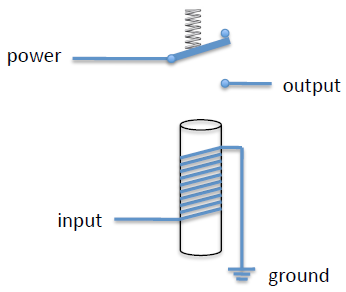
\includegraphics[scale=0.22]{figures/em_switch.png}

\smallskip

\tiny An electromechanical switch
\end{center}

\bigskip

Devices (\lstinline{AND} and \lstinline{OR} gates) for computing $x$ \lstinline{AND} $y$ and $x$ \lstinline{OR} $y$, constructed using electromechanical switches:
\begin{center}
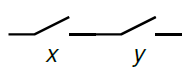
\includegraphics[scale=0.22]{figures/and_gate.png}\hspace{1cm} 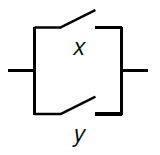
\includegraphics[scale=0.22]{figures/or_gate.png}

\smallskip

\tiny \lstinline{AND} and \lstinline{OR} gates
\end{center}

\bigskip

The function \lstinline{NOT} $x$ can be implemented by constructing a switch that conducts if and only $x$ is 0.
\end{frame}

\begin{frame}[fragile]
Computers today are built with transistorized switches that use the same principles as electromechanical switches, but are much smaller, much faster, more reliable, and more efficient. 

\bigskip

Since the details of the switches aren't terribly important at this level of abstraction, we represent, or ``abstract'', the gates using the following symbols:
\begin{center}
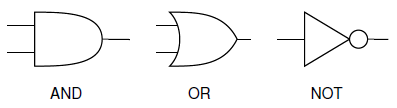
\includegraphics[scale=0.3]{figures/gate_symbols.png}

\smallskip

\tiny Symbols used for \lstinline{AND}, \lstinline{OR}, and \lstinline{NOT} gates
\end{center}

\bigskip

A logical circuit for the implication function $\bar{x}\bar{y}+\bar{x}y+xy$:
\begin{center}
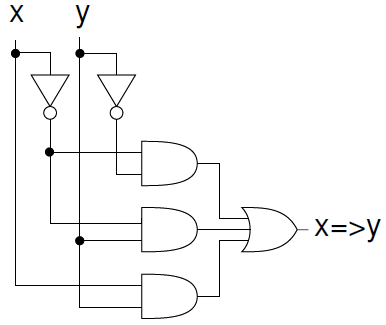
\includegraphics[scale=0.22]{figures/implication_circuit.png}

\smallskip

\tiny A circuit for the implication function
\end{center}
\end{frame}

\section{Computing With Logic}
\begin{frame}[fragile]
A truth table describing the addition of two two-bit numbers to get a three-bit result:
\begin{center}
\begin{tabular}{cc|c}
$x$ & $y$ & $x +y$ \\ \hline
00 & 00 & 000 \\
00 & 01 & 001 \\
00 & 10 & 010 \\
$\vdots$ & $\vdots$ & $\vdots$ \\
01 & 10 & 011 \\
01 & 11 & 100 \\
$\vdots$ & $\vdots$ & $\vdots$ \\
11 & 11 & 110
\end{tabular}
\end{center}
To build a corresponding circuit, we can apply the minterm expansion principle separately for each output bit, but this is infeasible --- adding two 16-bit numbers, for example, will result in a circuit with several billion gates.
\end{frame}

\begin{frame}[fragile]
We build a relatively simple circuit called a \emph{full adder} (FA) that does just one column of addition, and then we ``chain'' $n$ full adders together to add two $n$-bit numbers. The resulting circuit is called a \emph{ripple-carry adder}.
\begin{center}
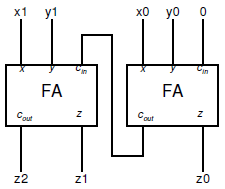
\includegraphics[scale=0.4]{figures/ripple_carry_adder.png}

\smallskip

\tiny A 2-bit ripple carry adder
\end{center}
\end{frame}

\section{Memory}
\begin{frame}[fragile]
Truth table for a \lstinline{NOR} gate (\lstinline{OR} followed by \lstinline{NOT}):
\begin{center}
\begin{tabular}{cc|c}
$x$ & $y$ & $x$ \lstinline$NOR$ $y$ \\ \hline
0 & 0 & 1 \\
0 & 1 & 0 \\
1 & 0 & 0 \\
1 & 1 & 0
\end{tabular}
\end{center}

\bigskip

A \emph{latch} is a device that allows us to ``lock'' a bit and retrieve it later. By aggregating millions of them we have the \emph{Random Access Memory (RAM)} that forms the memory of a computer.

\bigskip

A latch\footnote{A nice video on how an $S$-$R$ latch works: \href{https://www.youtube.com/watch?v=VtVIDgilwlA}{https://www.youtube.com/watch?v=VtVIDgilwlA}} can be constructed from two \lstinline{NOR} gates as shown below
\begin{center}
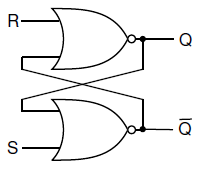
\includegraphics[scale=0.4]{figures/latch.png}

\smallskip

\tiny An $S$-$R$ latch built from two \lstinline{NOR} gates
\end{center}
where the input $S$ is known as ``set'' while the input $R$ is known as ``reset''.
\end{frame}

\section{von Neumann Architecture}
\begin{frame}[fragile]
In a modern computer, the \emph{CPU (Central Processing Unit)} is where all the computation takes place.

\bigskip

The CPU has devices such as ripple-carry adders, multipliers, etc. for doing arithmetic. In addition, it has a small amount of (scratch) memory called \emph{registers}.

\bigskip

The computer's main memory, which allows storing large amounts of data, is separate from the CPU and is connected to it by wires on the computer's circuit board.

\bigskip

A program, which is usually a long list of instructions, is stored in the main memory, and is copied, one instruction at a time, into a register in the CPU for execution.

\bigskip

The CPU has two special registers: a \emph{program counter} that keeps track of the location in memory where it will find the next instruction and an \emph{instruction register} that stores the next instruction to execute. 

\bigskip

This way of organizing computation is due to the famous mathematician and physicist, John von Neumann, and is known as the \emph{von Neumann architecture}.
\end{frame}

\begin{frame}[fragile]
Instructions, like data, can be encoded as numbers.

\bigskip

For example, let's assume our computer is based on 8-bit numbers and only has four instructions: add, subtract, multiply, and divide. Each of these instructions will need a number, called an \emph{operation code} (or \emph{opcode}), to represent it.
\begin{center}
\begin{tabular}{cc}
Opcode & Meaning \\ \hline
00 & Add \\
01 & Subtract \\ 
10 & Multiply \\
11 & Divide
\end{tabular}
\end{center}

\bigskip

Next, let's assume that our computer has four registers, numbered 0 through 3.

\bigskip

An instruction will be encoded using 8 bits as follows: the first two bits represent the instruction (operation), the next two bits encode the ``destination register'' where our result will be stored, the next two bits encode the register containing the first operand, and the last two bits encode the register containing the second operand. 

\bigskip

For example, the instruction \lstinline{add 3 0 2} (meaning add the contents of register 2 with the contents of register 0 and store the result in register 3) will be encoded as \lstinline{00110010}.
\end{frame}

\begin{frame}[fragile]
Our computer operates by repeatedly performing the following procedure:
\begin{enumerate}
\item Send the address in the program counter (commonly called the \emph{PC}) to the memory, asking it to read that location.

\item Load the value from memory into the instruction register.

\item \emph{Decode} the instruction register to determine what instruction to execute and which registers to use.

\item \emph{Execute} the requested instruction. This step often involves reading operands from registers, performing arithmetic, and sending the results back to the destination register. 

\item Increment PC so that it contains the address of the next instruction in memory.
\end{enumerate}
\begin{center}
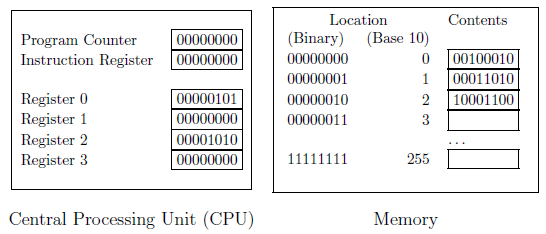
\includegraphics[scale=0.35]{figures/von_neumann_arch.png}

\smallskip

\tiny A computer with instructions stored in memory
\end{center}

\end{frame}
\end{document}
